\documentclass[12pt]{article}
\usepackage{graphicx}
\usepackage{enumitem}
\usepackage{amsmath}
\usepackage{gvv-book}
\usepackage{gvv}

\title{\textbf{2.7.20}}
\author{\textbf{EE25BTECH11008 - Anirudh M Abhilash}}
\date{September 16, 2025}

\begin{document}

\maketitle

\section*{Question}

The two adjacent sides of a parallelogram are 
\begin{align*}
\vec{a} = \myvec{2 \\ -4 \\ -5},  
\vec{b} = \myvec{2 \\ 2 \\ 3}
\end{align*}
Find the two unit vectors parallel to its diagonals. Using the diagonal vectors, find the area of the parallelogram.

\section*{Solution}

Diagonals:
\begin{align}
\vec{d}_1 = \vec{a} + \vec{b} \\
\vec{d}_2 = \vec{a} - \vec{b} \\
\vec{d}_1 = \myvec{4 \\ -2 \\ -2} \\ 
\vec{d}_2 = \myvec{0 \\ -6 \\ -8} 
\end{align}

Norms:
\begin{align}
\|\vec{d}_1\|^2 = \vec{d}_1^\top \vec{d}_1 = 24 \\
\|\vec{d}_1\| = 2\sqrt{6} \\
\|\vec{d}_2\|^2 = \vec{d}_2^\top \vec{d}_2 = 100 \\
\|\vec{d}_2\| = 10
\end{align}

Unit vectors along diagonals:
\begin{align}
\vec{u}_1 = \frac{\vec{d}_1}{\|\vec{d}_1\|}
= \frac{1}{2\sqrt{6}}\myvec{4 \\ -2 \\ -2} \\
\vec{u}_2 = \frac{\vec{d}_2}{\|\vec{d}_2\|} 
= \frac{1}{10}\myvec{0 \\ -6 \\ -8}.
\end{align}

Area of the parallelogram:
\begin{align}
\|\vec{a}\times\vec{b}\|^2 
= (\vec{a}^\top\vec{a})(\vec{b}^\top\vec{b}) - (\vec{a}^\top\vec{b})^2.
\\
\vec{a}^\top\vec{a} = 45, 
\quad 
\vec{b}^\top\vec{b} = 17, 
\quad 
\vec{a}^\top\vec{b} = -19.
\\
\|\vec{a}\times\vec{b}\|^2 = 45 \cdot 17 - (-19)^2 = 404,
\\
\text{Area} = \sqrt{404} = 2\sqrt{101}.
\end{align}

\begin{align*}
\boxed{\vec{u}_1 = \tfrac{1}{2\sqrt{6}}\myvec{4 \\ -2 \\ -2}, 
\quad 
\vec{u}_2 = \tfrac{1}{10}\myvec{0 \\ -6 \\ -8}, 
\quad 
\text{Area} = 2\sqrt{101}}
\end{align*}

\begin{figure}[H]\centering
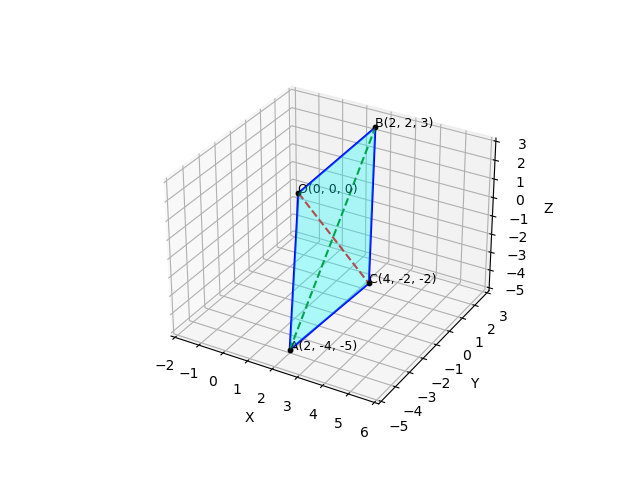
\includegraphics[width=1\columnwidth]{figs/plt.png}
\caption{Parallelogram along with diagonal vectors}
\label{fig:plt}
\end{figure}

\end{document}
